\resizebox{0.98\textwidth}{!}{%
\begin{tikzpicture}[
    x=1cm,
    y=1cm,
    >=Latex,
    line cap=round,
    line join=round,
    font=\sffamily,
    panel/.style={
        draw=#1!62,
        fill=#1!6,
        line width=0.75pt,
        rounded corners=7pt,
        minimum height=3.05cm,
        align=center
    },
    softpanel/.style={
        draw=#1!52,
        fill=#1!4,
        line width=0.65pt,
        dashed,
        rounded corners=7pt,
        align=center
    },
    card/.style={
        draw=#1!60,
        fill=white,
        line width=0.55pt,
        rounded corners=4pt,
        align=center,
        font=\scriptsize,
        inner sep=3pt
    },
    mutedcard/.style={
        draw=#1!40,
        fill=white,
        line width=0.45pt,
        rounded corners=4pt,
        align=center,
        font=\scriptsize,
        inner sep=3pt,
        text=black!70
    },
    tightcard/.style={
        draw=#1!60,
        fill=white,
        line width=0.55pt,
        rounded corners=4pt,
        align=center,
        font=\scriptsize,
        inner sep=1.4pt
    },
    flow/.style={->, line width=1.05pt, draw=blue!42},
    prelim/.style={->, line width=0.85pt, draw=gray!55},
    title/.style={font=\bfseries\scriptsize, text=#1!72!black, align=center},
    small/.style={font=\scriptsize, align=center},
    tinylabel/.style={font=\tiny\itshape, text=gray!68!black, align=center}
]

\definecolor{azulpaper}{RGB}{38,91,150}
\definecolor{naranjapaper}{RGB}{184,94,35}
\definecolor{moradopaper}{RGB}{92,68,143}
\definecolor{verdepaper}{RGB}{69,139,76}
\definecolor{doradopaper}{RGB}{176,127,38}
\definecolor{grisproy}{RGB}{112,123,134}

% Flujo principal: datos -> series -> conectividad -> comparacion -> visualizacion
\node[panel=azulpaper, minimum width=2.65cm] (datos) at (0,1.72) {};
\node[title=azulpaper] at (0,2.86) {Datos y atlas};
\node[card=azulpaper, minimum width=2.05cm, minimum height=0.50cm] at (0,2.36)
    {\textbf{ABIDE I}\\[-1pt]{\tiny rs-fMRI}};
\node[card=verdepaper, minimum width=2.05cm, minimum height=1.34cm] at (0,1.08) {};
\node[small, text=verdepaper!75!black] at (0,1.58) {\textbf{Schaefer 100}\\[-1pt]\textbf{ROIs}};
\node at (0,0.86) {
\includegraphics[height=0.84cm]{Img/pipeline_schaefer_rois_thumb.png}};

\node[panel=naranjapaper, minimum width=2.95cm] (series) at (3.15,1.72) {};
\node[title=naranjapaper] at (3.15,2.86) {Series temporales ROI};
\node[font=\scriptsize] at (3.15,2.42) {$\mathbf{X}\in\mathbb{R}^{T\times100}$};
\node[card=naranjapaper, minimum width=2.40cm, minimum height=1.28cm, inner sep=1pt] at (3.15,1.54) {};
\node at (3.15,1.54) {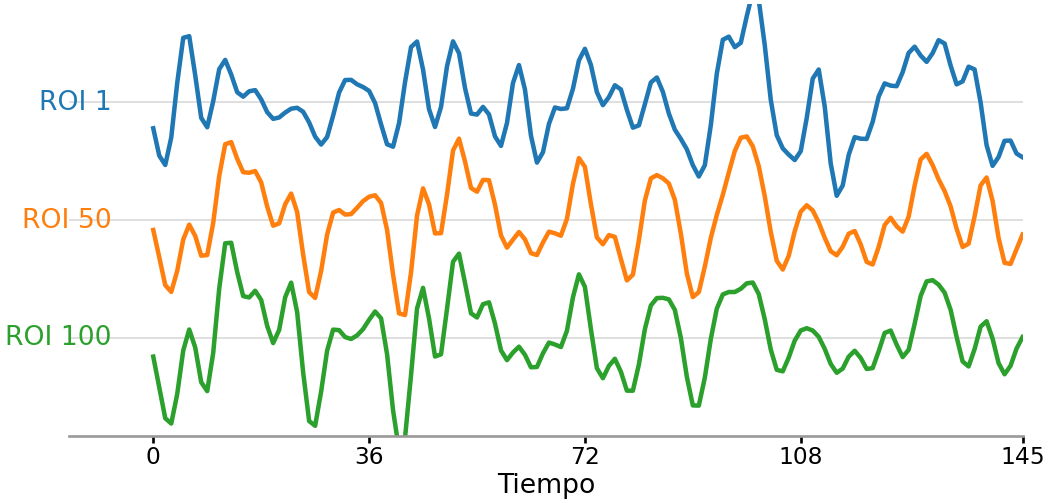
\includegraphics[width=2.25cm]{Img/pipeline_real_roi_series.png}};
\node[tinylabel] at (3.15,0.45) {se\~nales regionales z-score};

\node[panel=moradopaper, minimum width=3.35cm] (conect) at (6.65,1.72) {};
\node[title=moradopaper] at (6.65,2.88) {Estimaci\'on\\de conectividad};
\draw[dashed, draw=moradopaper!40, line width=0.60pt] (6.65,2.47) -- (6.65,0.86);
\node[font=\tiny\bfseries, text=azulpaper!75!black] at (5.88,2.30) {Asociativos};
\node[font=\tiny\bfseries, text=verdepaper!70!black, align=center] at (7.44,2.30) {Causal\\exploratorio};
\node[card=azulpaper, minimum width=1.28cm, minimum height=0.40cm] at (5.94,1.90) {Correlaci\'on};
\node[card=azulpaper, minimum width=1.28cm, minimum height=0.40cm] at (5.94,1.35) {Graphical\\Lasso};
\node[card=verdepaper, minimum width=1.28cm, minimum height=0.44cm] at (7.43,1.62) {LiNGAM};
\node[tinylabel] at (6.65,0.50) {matriz $100\times100$ por sujeto};

\node[panel=doradopaper, minimum width=3.02cm] (comparacion) at (10.15,1.72) {};
\node[title=doradopaper] at (10.15,2.88) {Comparaci\'on\\TEA y controles};
\node[tightcard=doradopaper, minimum width=2.28cm, minimum height=0.30cm] at (10.15,2.12) {Promedio controles};
\node[tightcard=doradopaper, minimum width=2.28cm, minimum height=0.30cm] at (10.15,1.66) {Promedio TEA};
\node[tightcard=doradopaper, minimum width=2.28cm, minimum height=0.40cm] at (10.15,1.16) {Diferencia\\TEA--controles};
\node[tightcard=doradopaper, minimum width=2.28cm, minimum height=0.30cm] at (10.15,0.63) {Conexiones top-20};
\node[tinylabel] at (10.15,0.28) {resumen visual descriptivo};

\node[panel=verdepaper, minimum width=2.75cm] (visual) at (13.35,1.72) {};
\node[title=verdepaper] at (13.35,2.86) {Visualizaci\'on};
\node[card=verdepaper, minimum width=2.00cm, minimum height=0.34cm] at (13.35,2.26) {Matrices promedio};
\node[card=verdepaper, minimum width=2.00cm, minimum height=0.34cm] at (13.35,1.70) {Mapas de diferencia};
\node[card=verdepaper, minimum width=2.00cm, minimum height=0.34cm] at (13.35,1.14) {Conectomas top-20};
\node[tinylabel] at (13.35,0.54) {resultados descriptivos};

% Clasificacion
\node[softpanel=grisproy, minimum width=8.85cm, minimum height=1.65cm] (posterior) at (7.55,-1.46) {};
\node[font=\bfseries\scriptsize, text=grisproy!85!black] at (7.55,-0.78)
    {Clasificaci\'on supervisada};
\node[mutedcard=grisproy, minimum width=1.60cm, minimum height=0.44cm] (vec) at (4.55,-1.48)
    {Vectorizaci\'on};
\node[mutedcard=grisproy, minimum width=1.86cm, minimum height=0.44cm] (clf) at (7.55,-1.48)
    {SVM RBF /\\Random Forest};
\node[mutedcard=grisproy, minimum width=2.45cm, minimum height=0.44cm] (met) at (10.55,-1.48)
    {Balanced accuracy, AUC};
\node[tinylabel] at (10.55,-2.00) {IC95\%, sensibilidad y especificidad};

% Flechas del flujo principal
\draw[flow] (1.37,1.72) -- (1.66,1.72);
\draw[flow] (4.68,1.72) -- (4.92,1.72);
\draw[flow] (8.38,1.72) -- (8.62,1.72);
\draw[flow] (11.70,1.72) -- (11.92,1.72);

% Flechas de la etapa preliminar
\draw[dashed, line width=0.80pt, draw=gray!50] (6.65,0.12) -- (6.65,-0.42) -| (4.55,-0.66);
\draw[prelim] (5.40,-1.48) -- (6.62,-1.48);
\draw[prelim] (8.48,-1.48) -- (9.30,-1.48);

\end{tikzpicture}%
}
